\documentclass[12pt, oneside]{article} 
\usepackage{amsmath, amsthm, amssymb, calrsfs, wasysym, verbatim, bbm, color, graphics, geometry}
\usepackage{hyperref}
\usepackage{standalone}

\geometry{tmargin=.75in, bmargin=.75in, lmargin=.75in, rmargin = .75in}  
\setlength{\parindent}{0in}
\setlength{\parskip}{\baselineskip}%
\setlength{\parindent}{1.5pt}%

\newcommand{\R}{\mathbb{R}}
\newcommand{\C}{\mathbb{C}}
\newcommand{\Z}{\mathbb{Z}}
\newcommand{\N}{\mathbb{N}}
\newcommand{\Q}{\mathbb{Q}}
\newcommand{\Cdot}{\boldsymbol{\cdot}}
\newcommand{\block}[1]{
  \underbrace{\begin{matrix}1 & \cdots & 1\end{matrix}}_{#1}
}
\newtheorem{thm}{Theorem}
\newtheorem{defn}{Definition}
\newtheorem{conv}{Convention}
\newtheorem{rem}{Remark}
\newtheorem{lem}{Lemma}
\newtheorem{cor}{Corollary}
\usepackage{tikz}  %TikZ central library is called.


\title{Lecture Note - 06: Tree, CART, Random Forest, Gradient Boosting Machine}
\author{Dihui Lai}

\begin{document}

\maketitle
\tableofcontents

\vspace{.25in}


%% normal frame
\section{Classification and Regression Tree (CART)}

\subsection{Impurity Measurement}
At node $\mathnormal{t}$, the fraction of class $\mathnormal{i}$ is denoted as $\mathnormal{p(i|t)}$
    
Entropy: $H(t)=-\sum\limits_{i=1}^{C}p(i|t)\log(p(i|t))$
    
Gini-Index: $Gini(t)=\sum\limits_{i=1}^{C}[p(i|t)]^2$
    
Classification Error: $Error(t)=1-\max\limits_{i}p(i|t)$

Considering the entropy of a data set that contains two types of outcomes: {0, 1}. Running 10 experiments, we get the following out comes (0, 0, 1, 0, 1, 0, 1, 1, 0, 1). The entropy is 
$$
\mathnormal{ H(t)}=-\sum\limits_{i=1}^{2}\frac{1}{2}\log_2(\frac{1}{2})=1
$$
    
What if we have out come of (1, 1, 1, 1, 1, 1, 1, 1, 1, 1)? The entropy is 
$$
\mathnormal{H(t)}=1\log_2(1)+0\log_2(0)=0
$$

The less variance in the data, the smaller the entropy is. For binary outcome, a probability of 1/2 leads to the largest uncertainty/entropy.

\subsection{Model}
John likes playing tennis on Saturday, The liklihood of John playing tennis depends on the weather. John has never played on a rainy. He may or may not play on a windy day. Given the weather, can you predict if John will play tennis this weekend?

\begin{figure}
\center
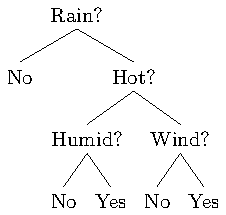
\includegraphics[scale=1.2,page=1]{Figures/CART.pdf}
\end{figure}

\subsection{Model: How to Grow a Tree?}
\begin{itemize}
\item At each node, the tree algorithm will check every variable for a possible split. 
\item A variable is selected for the split if it maximally reduces the impurity in the child nodes (e.g. the largest reduction of entroy, the largest reduction of variance etc.)
\item Pruning: a tree can grow till each leave only contains one data point. Pruning the tree is needed to avoid overfitting.
\end{itemize}

Stopping criterion
\begin{itemize}
\item[-] The number of training sample after split is less than certain number 'min\_ samples\_ split'.
\item[-] When the depth of the tree reaches to certain threshold 'max\_ depth'.
\end{itemize}

\subsection{ Gain at a Split Node}
Assuming we collect John's tennis activities for 20 weeks. Out of the 20 weekends, we have 8 sunny day and John plays tennis on all of them. Out of the rest 12 days, John played tennis on 7 days. 
Before any split, we have the entropy calculated as 
$$
\mathnormal{H(root)}=-\frac{15}{20}\log(\frac{15}{20})-\frac{5}{20}\log(\frac{5}{20})=0.562
$$

Split based on the weather, we have on sunny days
$
 \mathnormal{H(sunny)=0}
$
and on other days
$
\mathnormal{H(!sunny)}=-\frac{7}{12}\log(\frac{7}{12})-\frac{5}{12}\log(\frac{5}{12})=0.679
$
Therefore the child nodes have average entropy of 
$$
\mathnormal{H(childs)}=\frac{8}{20}\cdot 0+\frac{12}{20}\cdot 0.679=0.407
$$
We have entropy reduced by $\mathnormal{\Delta H}=0.562-0.390=0.154$

Instead of splitting by forcast, we look at the wind speed. Out of the 20 weekends, 10 days are windy and 10 days are not windy. Out of the windy day, John played 6 times and 9 times for the non-windy days.

Split based on the wind condition, we have on windy days
$
\mathnormal{H(!windy)}=-\frac{6}{10}\log(\frac{6}{10})-\frac{4}{10}\log(\frac{4}{10})=0.673
$
and on other days
$
\mathnormal{H(windy)}=\frac{9}{10} \log(\frac{9}{10})+\frac{1}{10} \log(\frac{1}{10})=0.325
$

Therefore the child nodes have average entropy of 
$$
\mathnormal{H(childs)}=\frac{1}{2} 0.673+\frac{1}{2} 0.325=0.499
$$
We have entropy reduced by $\mathnormal{\Delta H}=0.562-0.5=0.063$




\section{Random Forest}

It terms out that multiple trees together can produce better model than a single tree. 

In order to build a random forest, do the following to grow each individual tree.
\begin{itemize}
\item  use a random sub-sample with replacement, to grow each individual tree.
\item  At each node,  $\mathnormal{M<<m}$ columns are randomly selected, out of all m predictors. Usually, the default choice of $\mathnormal{M=m/3}$ for regression tree and $\mathnormal{M=\sqrt{m}}$ for classification tree.
\item Each tree is grown to the largest extent possible (one sample in the leaves)

\end{itemize}

\section{GBM}

The Gradient boosting tree is a collection of trees, where each individual tree is constructed to predict the 'residuals'.
$\mathnormal{\hat{y}(x_i)=\sum\limits_{k=1}^K \gamma_k h_k(x_i)}$, where $\mathnormal{h_k(x)}$ is a tree. 

The $\mathnormal{k^{th}}$ tree is built to fit the 'residuals' from the precedent $\mathnormal{k-1}$ trees  

The algorithm in a nutshell

Step 1: 
$$\mathnormal{\hat{y}_0(x) = \underset{\gamma}{\arg\min} \sum_{i=1}^n L(y^i, \gamma)}$$

Step 2: Fit a tree model $\mathnormal{h_{k}}$ by training it on the dataset $\mathnormal{[\vec{x}^i, r^{i}_{k}]}$

Here,
$$\mathnormal{r^{i}_{k} = -\left[\frac{\partial L(y^i, {y}(x^i))}{\partial y(x^i)}\right]_{{y}(x)=\hat{y}_{k-1}(x)} \quad \mbox{for } i=1,\ldots,n.}$$

Step 3: Update the estimator $\mathnormal{\hat{y}_{k}(x)=\hat{y}_{{k-1}}(x)+\gamma _{k}h_{k}(x)}$ 

Here, 
$\mathnormal{\gamma_k = \underset{\gamma}{\operatorname{arg\,min}} \sum_{i=1}^n L\left(y^i, \hat{y}_{k-1}(x^i) + \gamma h_k(x^i)\right)}$

Reference: 

\href{https://homes.cs.washington.edu/~tqchen/pdf/BoostedTree.pdf}{Xgboost}

\end{document}

